\documentclass[a4paper]{article} % For LaTeX2e
\usepackage[T1]{fontenc} % add special characters (e.g., umlaute)
\usepackage[utf8]{inputenc} % set utf-8 as default input encoding
\usepackage{ISMIRlbd, cite, times, amsmath, url}
\usepackage{hyperref}
\usepackage{url}
\usepackage{float}
\usepackage{graphicx}
\usepackage{booktabs}
\usepackage{color}

\usepackage{booktabs}       % lepší vodorovné linky v tabulkách
\usepackage{xcolor}
\usepackage{colortbl}

\title{Melody Extraction using a Harmonic CNN}


% Note: Please do NOT use \thanks or a \footnote in any of the author markup

% Single address
% To use with only one author or several with the same address
% ---------------
%\oneauthor
% {Names should be omitted for double-blind reviewing}
% {Affiliations should be omitted for double-blind reviewing}

% Two addresses
% --------------
\twoauthors
 {Jiří Balhar} {Charles University \\ Institute of Formal and Applied Linguistics}
 {Jan Hajič jr.} {Charles University \\ Institute of Formal and Applied Linguistics}

%% To make customize author list in Creative Common license, uncomment and customize the next line
%  \def\authorname{First Author, Second Author}

% \threeauthors
%   {First Author} {Affiliation1 \\ {\tt author1@ismir.edu}}
%   {Second Author} {Affiliation2 \\ {\tt author2@ismir.edu}}
%   {Third Author} {Affiliation3 \\ {\tt author3@ismir.edu}}


\newcommand{\fix}{\marginpar{FIX}}
\newcommand{\new}{\marginpar{NEW}}

%\iclrfinalcopy % Uncomment for camera-ready version, but NOT for submission.
\begin{document}


\maketitle

\begin{abstract}


In the recent years the approaches to melody extraction have shifted to the use of deep learning (DL). These new methods transform the input signal to a time-frequency representation and then use DL techniques to sequentially process the transformed input. The result is a saliency map from which they select the melody $f_0$ trajectory and determine voicing. Among new DL-based works we can find variety of approaches that try new signal transformations or network topologies; on the other hand the building blocks out of which these systems are built are standard (fully connected layers, CNNs and RNNs) \cite{Kum2016,Rigaud2016,Bittner2017,DBasaranSEssid2018}. In this paper we propose a new kind of CNN layer specialized for processing harmonic signals in audio.

% 
% Ordinary CNNs are not well suited for processing such data since they are not able to process the whole harmonic structure in one layer. 
%The use of ordinary CNNs for processing audio data has a major limitation. 
A harmonic signal is usually comprised of a fundamental frequency and overtones that are spaced apart by constant ratios. These features are therefore non-local on a input time-frequency representation. In practice CNN kernels are usually small (previous works use usually a size of a semitone in the frequency axis \cite{Bittner2017,DBasaranSEssid2018}) and therefore cannot process the whole harmonic structure in one layer. To make up for this, existing works also include a final "big" convolutional layer to "capture relationships between frequency content within a octave" \cite{Bittner2017}. This is only a partial solution because only one layer of the whole network can exploit the defining characteristic of a harmonic signal.

\begin{figure}[H]
 \centerline{\framebox{
 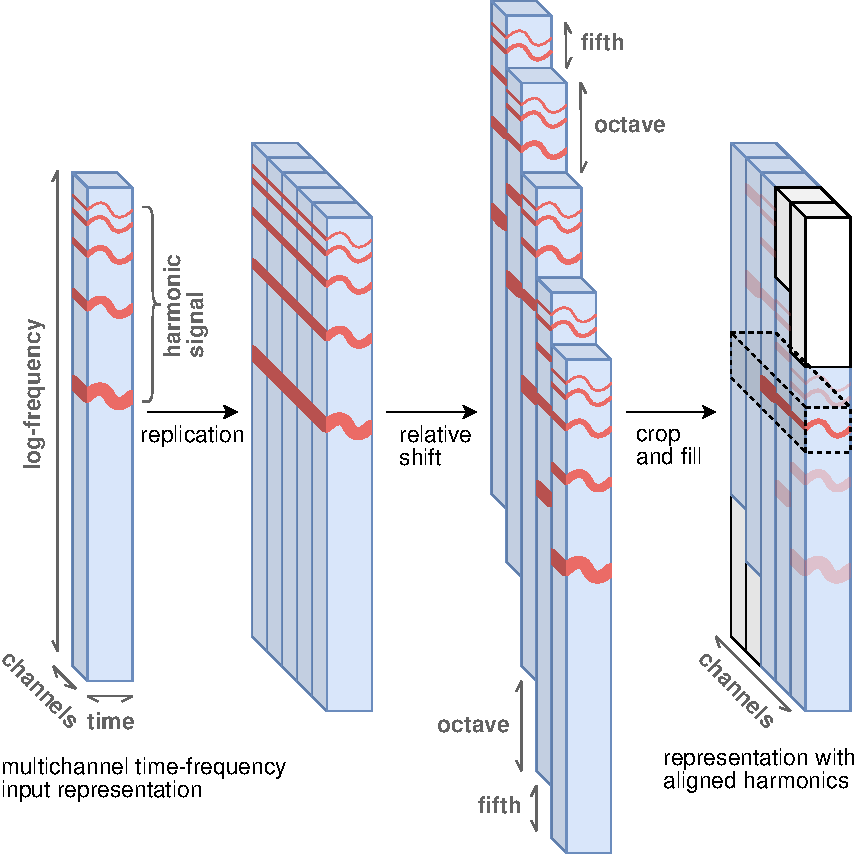
\includegraphics[width=0.38\columnwidth]{hcnn_transform_en_2}}}
 \caption{Diagram of the input transformation for convolution layers.}
 \label{fig:hcnn_transform}
\end{figure}

% The architecture has the standard overall structure of processing an input through a series of convolutional layers

Our proposed Harmonic Convolutional Neural Network (HCNN) overcomes this limitation.\footnote{For the source code please see the accompanying repository at \url{https://github.com/kukas/music-transcription}} The convolutional layer in our network is able to use all the relevant harmonic information in each layer. Our architecture has the standard structure of processing an input through a series of convolutional layers similar to \cite{Bittner2017}. Crucially before each convolutional layer we add an additional transformation of the input (see \figref{fig:hcnn_transform}). 

The transformation first creates copies of the input and stacks them in the channel axis. We then shift these copies relative to the original in the frequency axis so that the information about harmonically related peaks are positioned above the original fundamental frequency. For a log-frequency spectrogram, the offsets are constant. This transformed input is then fed into the next convolutional layer. Since the convolutional filter has the access to all channels, it follows that it has access to the provided harmonically related information for every time-frequency position in the matrix.

We train two architectures on a subset of MedleyDB. HCNN noctx which uses only $\approx 5.5\,\rm ms$ window of input audio for the melody estimation and HCNN ctx which uses $\approx 162.4\,\rm ms$ (comparable to Bittner et al. \cite{Bittner2017}). We compare these with state-of-the-art baselines: "SAL" \cite{Salamon2012a}, "BIT" \cite{Bittner2017} and "BAS" \cite{DBasaranSEssid2018}. In case of BIT and BAS, we ran the algorithms using the source code obtained from the links provided in the papers keeping default parameters. For the SAL algorithm we used the implementation in Essentia library \footnote{\url{https://essentia.upf.edu}}.

As testing data we use MedleyDB test set, ADC04 dataset, MIREX05 training set \footnote{We downloaded ADC04 and MIREX05 datasets from \url{https://labrosa.ee.columbia.edu/projects/melody/}}, Orchset \cite{Bosch2016}, a subset of MDB-melody-synth \cite{Salamon2017} and a subset of WJAZZD \cite{Pfleiderer}. For the complete list of selected testing tracks please see our code repository.



\begin{table}[H]
\centering
\scalebox{0.8}{%
\begin{tabular}{lrrrrrr}
\toprule
Method & ADC04 & \shortstack[r]{MDB-m-s\\ test} & \shortstack[r]{MIREX05\\train.} & \shortstack[r]{MDB\\test} & \shortstack[r]{ORCH-\\SET} & \shortstack[r]{WJazzD\\test} \\
\midrule
    SAL &         0.714 &           0.527 &          0.715 &         0.519 &        0.235 &        0.667 \\
    BIT &         0.716 &           0.633 &          0.702 &         0.611 &        0.407 &        0.692 \\
    BAS &         0.669 &   \textbf{0.689}&          0.734 &         0.640 &\textbf{0.483}&        0.700 \\
\arrayrulecolor{black!30}\midrule
 \shortstack[l]{HCNN noctx} & \textbf{0.737}&           0.626 &          0.723 &         0.635 &        0.439 &        0.715 \\
 \shortstack[l]{HCNN ctx}   &         0.726 &           0.661 &  \textbf{0.755}& \textbf{0.652}&        0.459 &\textbf{0.725} \\
\arrayrulecolor{black}\bottomrule
\end{tabular}
}%
\caption{Overall Accuracy of the selected methods. Highlighted values are the highest across the dataset.}\label{tab:results_OA}
\end{table}

Our methods outperform all selected baselines on four out of six testing datasets (see \tabref{tab:results_OA}). Compared to the most similar method BIT we achieve better results on all datasets with a gain of +3.6 percentage points in average on the Overall Accuracy (OA) metric while using almost 20 times less trainable parameters in the model. Based on these results we believe that the architecture has a potential in other related tasks such as multi-$f_0$ tracking.

\end{abstract}

%\subsubsection*{Acknowledgments}
\begin{acknowledgments}
We would like to thank the Jazzomat Research Project for kindly providing the WJazzD testing data.
\end{acknowledgments}

\bibliography{ISMIRtemplate}
%\bibliographystyle{iclr2019_conference}

\end{document}
